% Copyright 2004 by Till Tantau <tantau@users.sourceforge.net>.
%
% In principle, this file can be redistributed and/or modified under
% the terms of the GNU Public License, version 2.
%
% However, this file is supposed to be a template to be modified
% for your own needs. For this reason, if you use this file as a
% template and not specifically distribute it as part of a another
% package/program, I grant the extra permission to freely copy and
% modify this file as you see fit and even to delete this copyright
% notice. 

\documentclass{beamer}

\usepackage{graphicx}

% There are many different themes available for Beamer. A comprehensive
% list with examples is given here:
% http://deic.uab.es/~iblanes/beamer_gallery/index_by_theme.html
% You can uncomment the themes below if you would like to use a different
% one:
%\usetheme{AnnArbor}
%\usetheme{Antibes}
%\usetheme{Bergen}
%\usetheme{Berkeley}
%\usetheme{Berlin}
%\usetheme{Boadilla}
%\usetheme{boxes}
%\usetheme{CambridgeUS}
%\usetheme{Copenhagen}
%\usetheme{Darmstadt}
%\usetheme{default}
%\usetheme{Frankfurt}
%\usetheme{Goettingen}
%\usetheme{Hannover}
%\usetheme{Ilmenau}
%\usetheme{JuanLesPins}
%\usetheme{Luebeck}
%\usetheme{Madrid}
%\usetheme{Malmoe}
%\usetheme{Marburg}
%\usetheme{Montpellier}
%\usetheme{PaloAlto}
%\usetheme{Pittsburgh}
%\usetheme{Rochester}
\usetheme{Singapore}
%\usetheme{Szeged}
%\usetheme{Warsaw}

\addtobeamertemplate{navigation symbols}{}{%
    \usebeamerfont{footline}%
    \usebeamercolor[fg]{footline}%
    \hspace{1em}%
    \insertframenumber/\inserttotalframenumber
}

\title{Towards Nonmonotonic Relational Learning from Knowledge Graphs}

% A subtitle is optional and this may be deleted
\subtitle{}

\author{Hai Dang Tran\inst{1}}
% - Give the names in the same order as the appear in the paper.
% - Use the \inst{?} command only if the authors have different
%   affiliation.

\institute[Max Planck Institute for Informatics] % (optional, but mostly needed)
{
  \inst{1}%
  Saarland University\\
  Max Planck Institute for Informatics
}
% - Use the \inst command only if there are several affiliations.
% - Keep it simple, no one is interested in your street address.

\date{2016}
% - Either use conference name or its abbreviation.
% - Not really informative to the audience, more for people (including
%   yourself) who are reading the slides online

\subject{Theoretical Computer Science}
% This is only inserted into the PDF information catalog. Can be left
% out. 

% If you have a file called "university-logo-filename.xxx", where xxx
% is a graphic format that can be processed by latex or pdflatex,
% resp., then you can add a logo as follows:

% \pgfdeclareimage[height=1cm]{university-logo}{mpi-logo.png}
% \logo{\pgfuseimage{university-logo}}

% Delete this, if you do not want the table of contents to pop up at
% the beginning of each subsection:
\AtBeginSubsection[]
{
  \begin{frame}<beamer>{Outline}
    \tableofcontents[currentsection,currentsubsection]
  \end{frame}
}

% Let's get started
\begin{document}

\begin{frame}
  \titlepage
\end{frame}

\begin{frame}{Outline}
  \tableofcontents
  % You might wish to add the option [pausesections]
\end{frame}

% Section and subsections will appear in the presentation overview
% and table of contents.
\section{System Overview}

\begin{frame}{System Overview}

\begin{figure}[h]
	\centering
	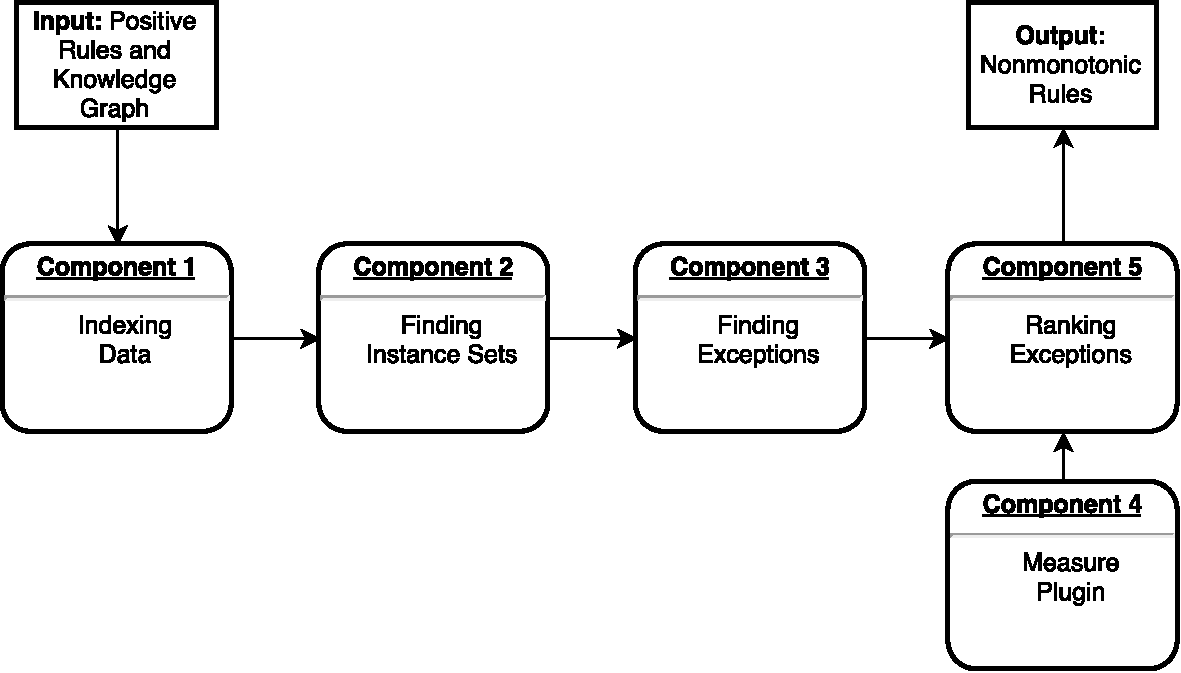
\includegraphics[page=1,width=.75\textwidth]{overview.pdf}
	\caption{Components in the System}
\end{figure}

\end{frame}

\section{System Description}

\subsection{Indexing Data}

\begin{frame}{System Description}{Indexing Data}

Given a knowledge graph $G$ as a list of \textit{$<$x p y$>$} triples.

\begin{itemize}
	\item {
    	We want to find a list of \textit{$<$p y$>$} given \textit{x}.
  	}
  	\item {   
    	Or a list of \textit{p} given \textit{$<$x, y$>$}.
	}
	\item {
		...
		\pause
	}
\end{itemize}

This is to support searching over a dataset.
\begin{itemize}
	\item Like indexing from term to document in IR systems.
  	\item In this problem, a triple is a document.
  	\item Combinatorial combination of \textit{x, p, y} can be a term.
\end{itemize}

\end{frame}

\subsection{Finding Instance Sets}

\begin{frame}{System Description}{Finding Instance Sets}

Assume that a given Horn rule $r$ is in the form: \textit{H(x, z) $\leftarrow$ P(x, y) $\wedge$ Q(y, z)}. How to find (ab)normal sets $NS(r)$, $ABS(r)$?
\begin{itemize}
	\item Enumerate variable $y$.
	\item Find list of $y$ from $Px$ based on indexing.
	\item Find list of $z$ from $Qy$ based on indexing.
	\item Check \textit{$<$x H z$>$} in the graph or not.
	\item Classify \textit{$<$x z$>$} into $NS(r)$ and $ABS(r)$.
\end{itemize}

\end{frame}

\subsection{Finding Exceptions}

\begin{frame}{System Description}{Finding Exceptions}

Three exception types:
\begin{itemize}
	\item $E_1(r), E_2(r)$ as unary predicates for $x$, $z$, resp.
	\item {
		$E_3(r)$ as binary predicate for $(x, z)$.
		\pause
	}
\end{itemize}

How to find $E_3(r)$?
\begin{itemize}
	\item Let $E_3^+(r) = \{P | \exists (x, z) \in ABS(r): P(x, z) \in G\}$.
	\item Let $E_3^-(r) = \{P | \exists (x, z) \in NS(r): P(x, z) \in G\}$.
	\item Then $E_3(r) = E_3^+(r) - E_3^-(r)$.
\end{itemize}

To find $E_3^+$, we use data indexing again.

\end{frame}

\subsection{Measure Plugin}

\begin{frame}{System Description}{Measure Plugin}
We need to test different measures:
\begin{itemize}
	\item Confidence measure is not good for prediction.
	\item Current measure is conviction, $conv(r) = (1 - supp(r)) / (1 - conf(r))$.
	\item Other measures can be plugged in the system.
\end{itemize}
\end{frame}

\subsection{Ranking Exceptions}

\begin{frame}{System Description}{Ranking Exceptions}

Ordered Partial Materialization (OPM):
\begin{itemize}
	\item Sort all positive rules according to decreasing order of conviction.
	\item For each rule $r$, we use original facts and predicted ones (updated KB) from previous rules to infer $NS(r), ABS(r)$.
	\item Find the list of possible exceptions for $r$.
	\item Rank exceptions based on conviction over updated KB.
	\item Choose all exceptions of $r$ to infer new facts.
\end{itemize}

\end{frame}

\section{Future Work}

\begin{frame}{Future Work}

Several works need to be done:

\begin{itemize}
	\item Extend experiment to YAGO.
	\item Enable more forms for given positive rules.
	\item Test with other predictive measures.
\end{itemize}

\end{frame}

%\section*{Summary}
%
%\begin{frame}{Summary}
%
%\appendix
%\section<presentation>*{\appendixname}
%\subsection<presentation>*{For Further Reading}
%
%\begin{frame}[allowframebreaks]
%  \frametitle<presentation>{For Further Reading}
%    
%  \begin{thebibliography}{10}
%    
%  \beamertemplatebookbibitems
%  % Start with overview books.
%
%  \bibitem{Author1990}
%    A.~Author.
%    \newblock {\em Handbook of Everything}.
%    \newblock Some Press, 1990.
% 
%    
%  \beamertemplatearticlebibitems
%  % Followed by interesting articles. Keep the list short. 
%
%  \bibitem{Someone2000}
%    S.~Someone.
%    \newblock On this and that.
%    \newblock {\em Journal of This and That}, 2(1):50--100,
%    2000.
%  \end{thebibliography}
%\end{frame}

\end{document}


